\documentclass[12pt]{article}
\usepackage{amsmath}
\usepackage{amsfonts}
\usepackage{graphicx}
\usepackage{geometry}
\usepackage{placeins} 

\geometry{a4paper, margin=1in}
\title{Unconstrained Optimization} 
\author{Gobinda Pandey, Image Adhikari}
\date{October 2024}

\begin{document}

\maketitle

\section{Introduction}
This report examines various optimization algorithms applied to three different problems. We employ Gradient Descent, Newton's Method, Quasi-Newton methods, and optionally the Adam method to minimize specific objective functions. We detail the solutions and performance of each method.

\section{Analysis of Optimization Methods}
\subsection*{Objective Function: Quadratic}
\begin{table}[htbp]
   \centering
   \small % Reduce font size
   \begin{tabular}{|c|c|c|}
      \hline
      \textbf{Method} & \textbf{Steps} & \textbf{Minimum \( f(x) \)} \\
      \hline
      Gradient Descent & \textit{85} & \textit{0.025517836989300404} \\
      \hline
      Newton's Method & \textit{1} & \textit{0.0} \\
      \hline
      Quasi-Newton Method (BFGS) & \textit{73} & \textit{0.012437960354649474} \\
      \hline
      Adam Method (Optional) & \textit{3247} & \textit{0.026126965235065427} \\
      \hline
   \end{tabular}
   \caption{\small Optimization results for the Quadratic Function}
   \label{tab:quadratic_function_results}
\end{table}

\begin{figure}[htbp]
   \centering
   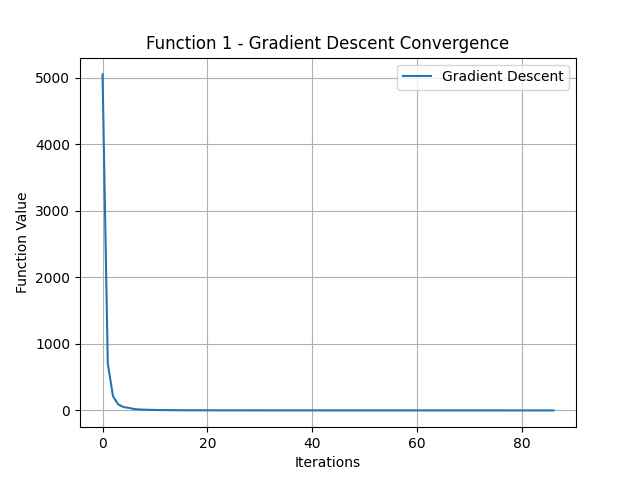
\includegraphics[width=0.18\textwidth]{/home/gobinda/My_Courses/QF/Optimization_Project2/artifacts/function_1_gradient_descent_convergence.png}
   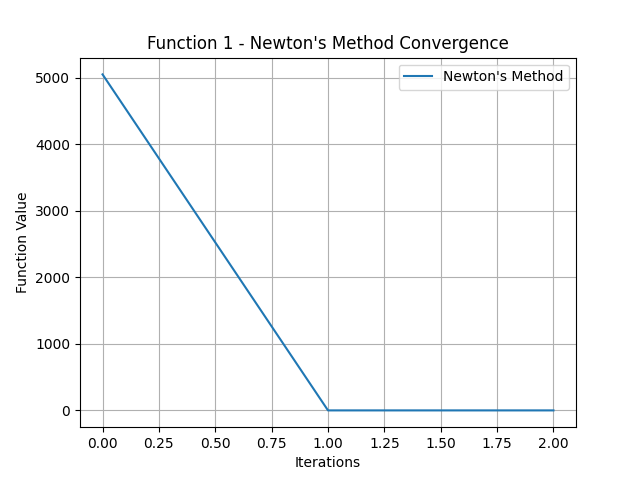
\includegraphics[width=0.18\textwidth]{/home/gobinda/My_Courses/QF/Optimization_Project2/artifacts/function_1_newton's_method_convergence.png}
   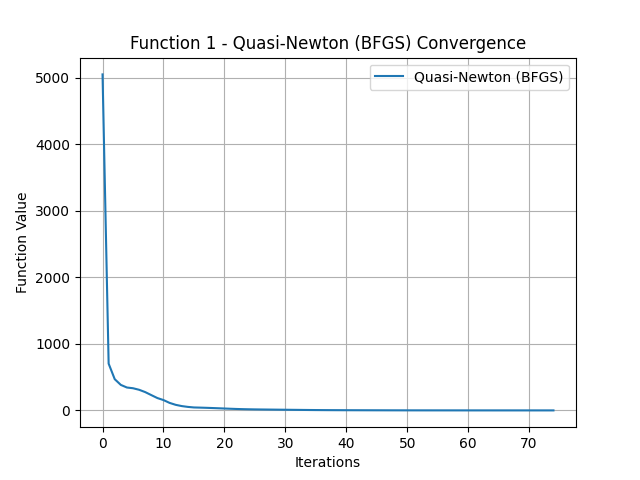
\includegraphics[width=0.18\textwidth]{/home/gobinda/My_Courses/QF/Optimization_Project2/artifacts/function_1_quasi-newton_(bfgs)_convergence.png}
   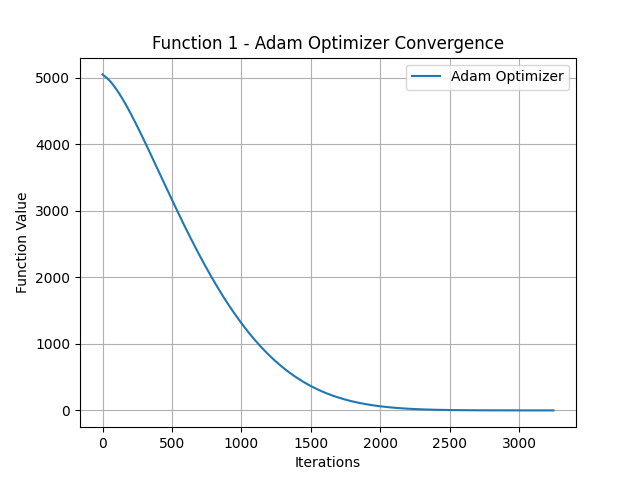
\includegraphics[width=0.18\textwidth]{/home/gobinda/My_Courses/QF/Optimization_Project2/artifacts/function_1_adam_optimizer_convergence.png}
   \caption{\small Convergence results for the Quadratic Function}
   \label{fig:quadratic_function_convergence}
\end{figure}

\begin{figure}[htbp]
   \centering
   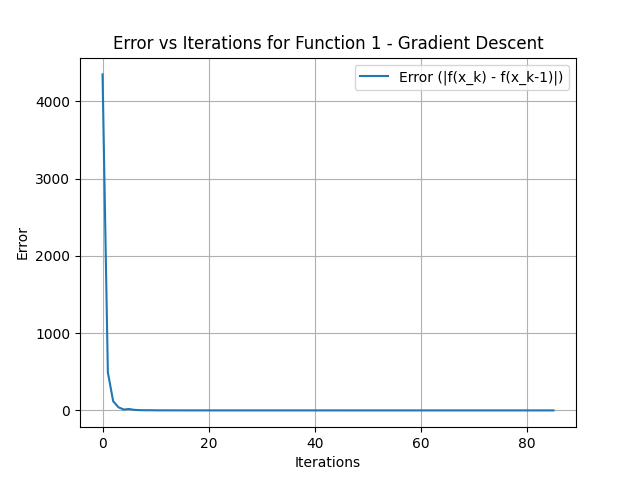
\includegraphics[width=0.18\textwidth]{/home/gobinda/My_Courses/QF/Optimization_Project2/artifacts/function_1_gradient_descent_errors.png}
   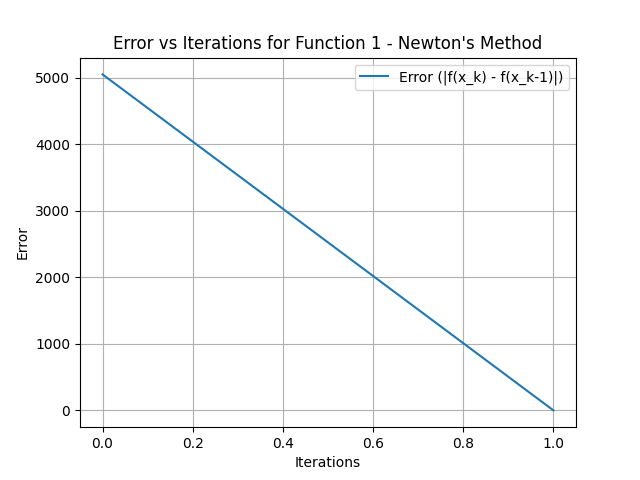
\includegraphics[width=0.18\textwidth]{/home/gobinda/My_Courses/QF/Optimization_Project2/artifacts/function_1_newton's_method_errors.png}
   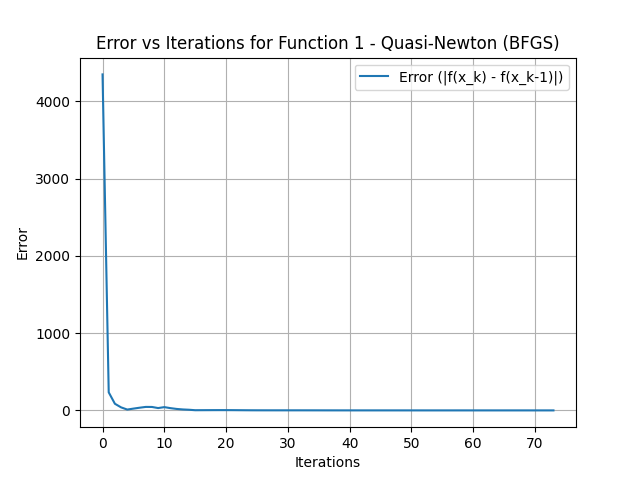
\includegraphics[width=0.18\textwidth]{/home/gobinda/My_Courses/QF/Optimization_Project2/artifacts/function_1_quasi-newton_(bfgs)_errors.png}
   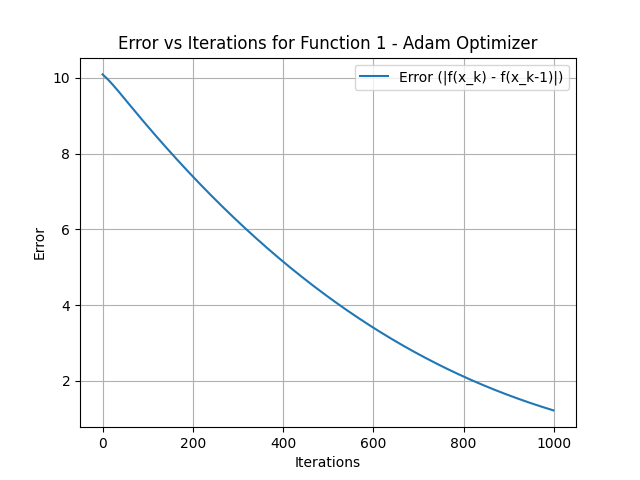
\includegraphics[width=0.18\textwidth]{/home/gobinda/My_Courses/QF/Optimization_Project2/artifacts/function_1_adam_optimizer_errors.png}
   \caption{\small Error results for the Quadratic Function}
   \label{fig:quadratic_function_errors}
\end{figure}

\subsubsection*{Explanation}
The quadratic function is convex, making it suitable for all optimization methods. \textbf{Table \ref{tab:quadratic_function_results}} shows that Newton's Method achieved the minimum in one step, demonstrating high efficiency. Gradient Descent required 85 steps, while Adam needed 3247 steps, indicating slower convergence. The Quasi-Newton Method (BFGS) performed well, converging in 73 steps.
\textbf{Figure \ref{fig:quadratic_function_convergence}} illustrates convergence behavior. Newton's Method quickly reaches the minimum, while Gradient Descent and Adam show gradual convergence. BFGS offers a middle ground with relatively fast convergence.
\textbf{Figure \ref{fig:quadratic_function_errors}} shows error reduction over iterations. Newton's Method and BFGS exhibit rapid error reduction, whereas Gradient Descent and Adam need more iterations for similar accuracy.

\subsection*{Objective Function: Log Barrier}

\begin{table}[htbp]
   \centering
   \small % Reduce font size
   \begin{tabular}{|c|c|c|}
      \hline
      \textbf{Method} & \textbf{Steps} & \textbf{Minimum \( f(x) \)} \\
      \hline
      Gradient Descent & \textit{877} & \textit{-2432.5708485843734} \\
      \hline
      Newton's Method & \textit{8} & \textit{-2432.866326777652} \\
      \hline
      Quasi-Newton Method (BFGS) & \textit{112} & \textit{-2432.8613348462163} \\
      \hline
      Adam Method (Optional) & \textit{8000} & \textit{-2431.104760050882} \\
      \hline
   \end{tabular}
   \caption{\small Optimization results for the Log Barrier Function}
   \label{tab:log_barrier_function_results}
\end{table}

\begin{figure}[htbp]
   \centering
   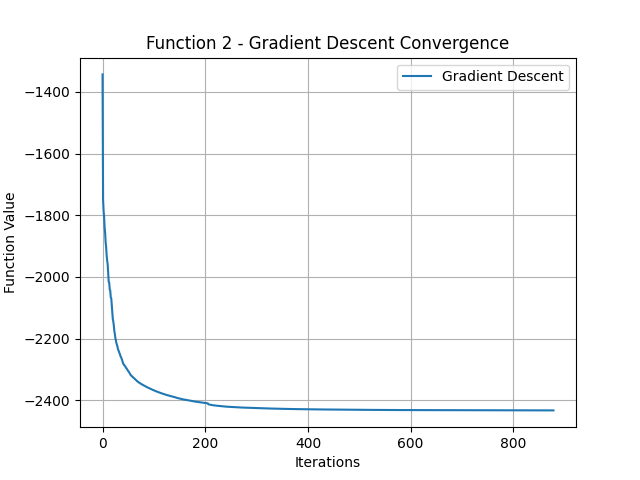
\includegraphics[width=0.18\textwidth]{/home/gobinda/My_Courses/QF/Optimization_Project2/artifacts/function_2_gradient_descent_convergence.png}
   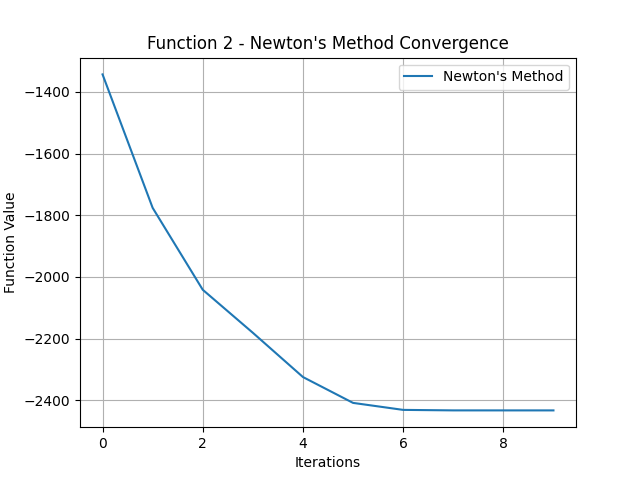
\includegraphics[width=0.18\textwidth]{/home/gobinda/My_Courses/QF/Optimization_Project2/artifacts/function_2_newton's_method_convergence.png}
   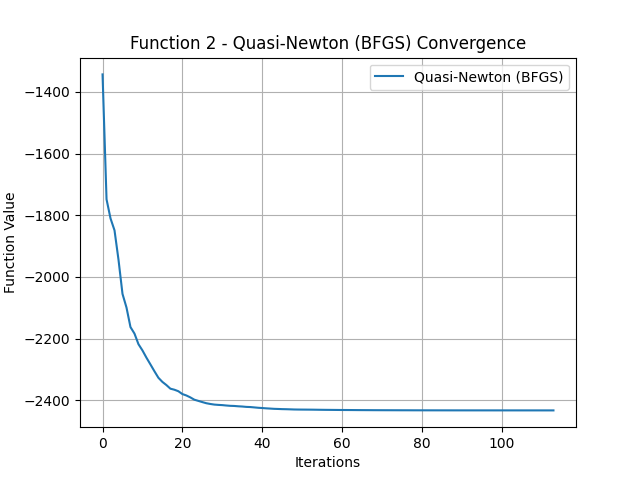
\includegraphics[width=0.18\textwidth]{/home/gobinda/My_Courses/QF/Optimization_Project2/artifacts/function_2_quasi-newton_(bfgs)_convergence.png}
   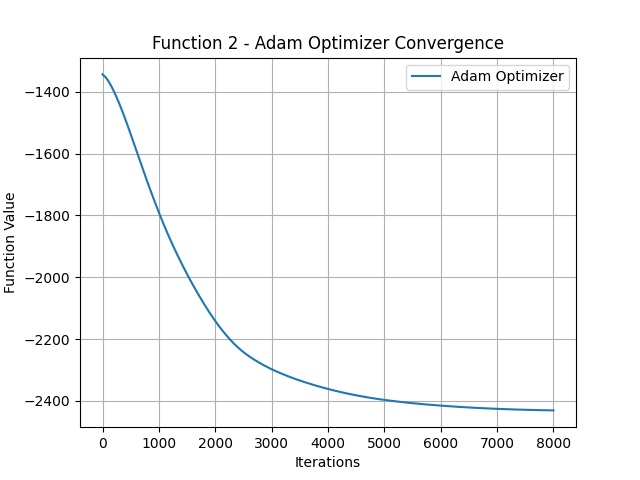
\includegraphics[width=0.18\textwidth]{/home/gobinda/My_Courses/QF/Optimization_Project2/artifacts/function_2_adam_optimizer_convergence.png}
   \caption{\small Convergence results for the Log Barrier Function}
   \label{fig:log_barrier_function_convergence}
\end{figure}

\begin{figure}[htbp]
   \centering
   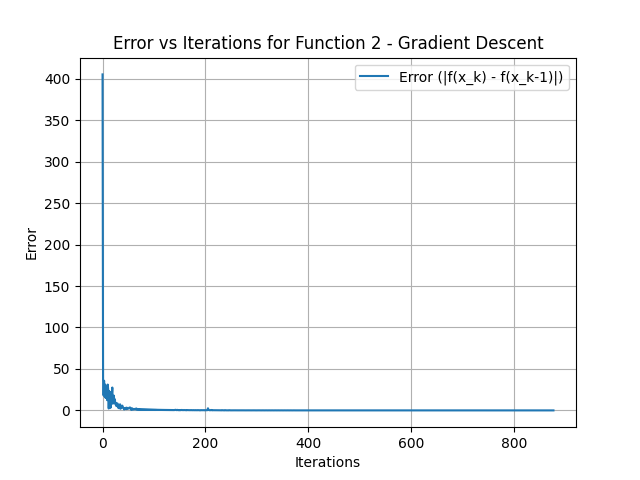
\includegraphics[width=0.18\textwidth]{/home/gobinda/My_Courses/QF/Optimization_Project2/artifacts/function_2_gradient_descent_errors.png}
   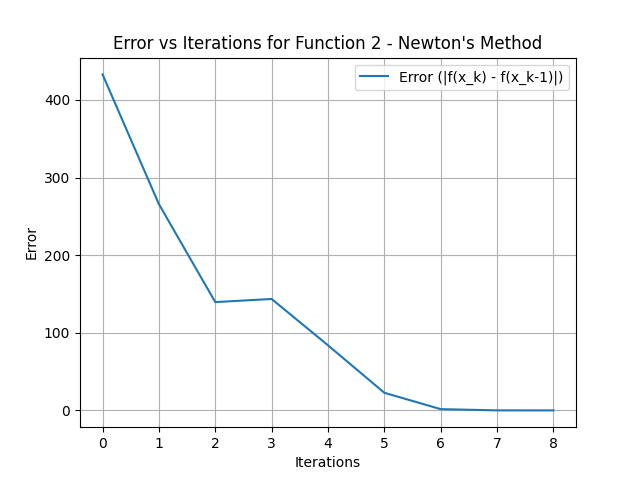
\includegraphics[width=0.18\textwidth]{/home/gobinda/My_Courses/QF/Optimization_Project2/artifacts/function_2_newton's_method_errors.png}
   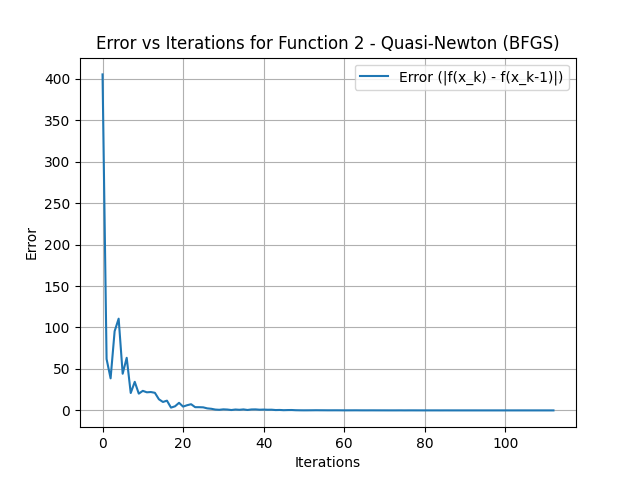
\includegraphics[width=0.18\textwidth]{/home/gobinda/My_Courses/QF/Optimization_Project2/artifacts/function_2_quasi-newton_(bfgs)_errors.png}
   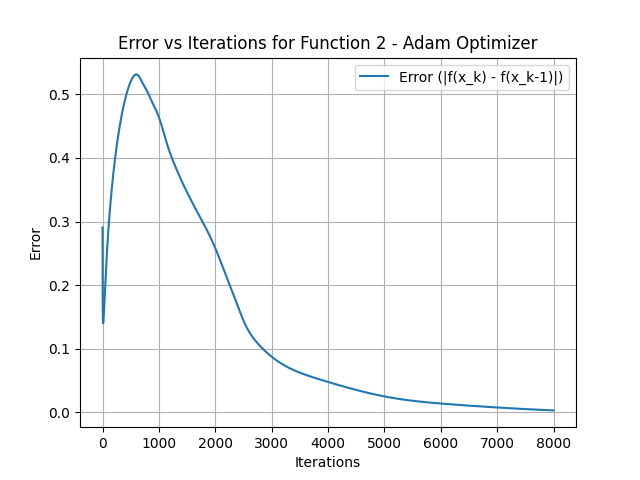
\includegraphics[width=0.18\textwidth]{/home/gobinda/My_Courses/QF/Optimization_Project2/artifacts/function_2_adam_optimizer_errors.png}
   \caption{\small Error results for the Log Barrier Function}
   \label{fig:log_barrier_function_errors}
\end{figure}

\FloatBarrier % Add this to ensure figures stay within the section

\subsubsection*{Explanation}
The log-barrier function introduces constraints, increasing complexity. \textbf{Table \ref{tab:log_barrier_function_results}} shows that Newton's Method achieved the minimum in 8 steps, demonstrating high efficiency. Gradient Descent and Adam required significantly more steps, converging in 877 and 8000 steps, respectively. The Quasi-Newton Method (BFGS) performed well, converging in 112 steps.
\textbf{Figure \ref{fig:log_barrier_function_convergence}} illustrates the convergence behavior. Newton's Method quickly reaches the minimum, while Gradient Descent and Adam show gradual convergence. BFGS balances between the two.
\textbf{Figure \ref{fig:log_barrier_function_errors}} shows error reduction over iterations. Newton's Method and BFGS exhibit rapid error reduction, whereas Gradient Descent and Adam need more iterations for similar accuracy.

\subsection*{Objective Function: Rosenbrock}

\begin{table}[htbp]
   \centering
   \small % Reduce font size
   \begin{tabular}{|c|c|c|}
      \hline
      \textbf{Method} & \textbf{Steps} & \textbf{Minimum \( f(x) \)} \\
      \hline
      Gradient Descent & \textit{3} & \textit{0.1997655255915457} \\
      \hline
      Newton's Method & \textit{10} & \textit{0.0005784005843096896} \\
      \hline
      Quasi-Newton Method (BFGS) & \textit{5} & \textit{0.053686336330168706} \\
      \hline
      Adam Method & \textit{1474} & \textit{0.7850856229011988} \\
      \hline
   \end{tabular}
   \caption{\small Optimization results for the Rosenbrock Function}
   \label{tab:rosenbrock_function_results}
\end{table}

\begin{figure}[htbp]
   \centering
   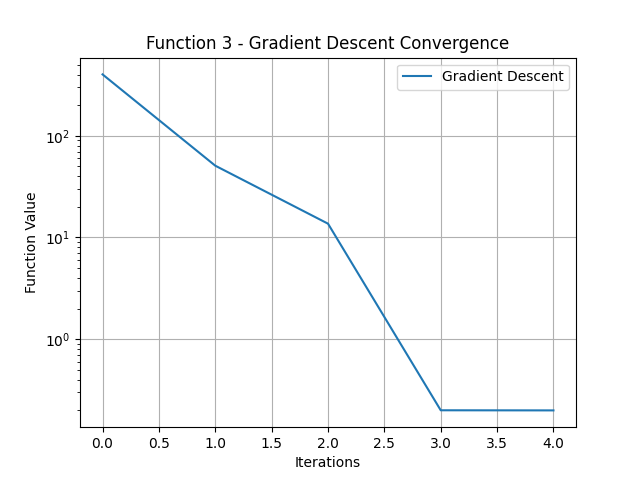
\includegraphics[width=0.18\textwidth]{/home/gobinda/My_Courses/QF/Optimization_Project2/artifacts/function_3_gradient_descent_convergence.png}
   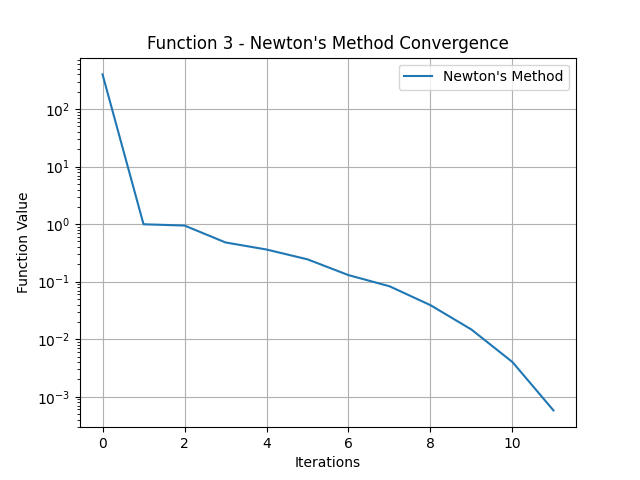
\includegraphics[width=0.18\textwidth]{/home/gobinda/My_Courses/QF/Optimization_Project2/artifacts/function_3_newton's_method_convergence.png}
   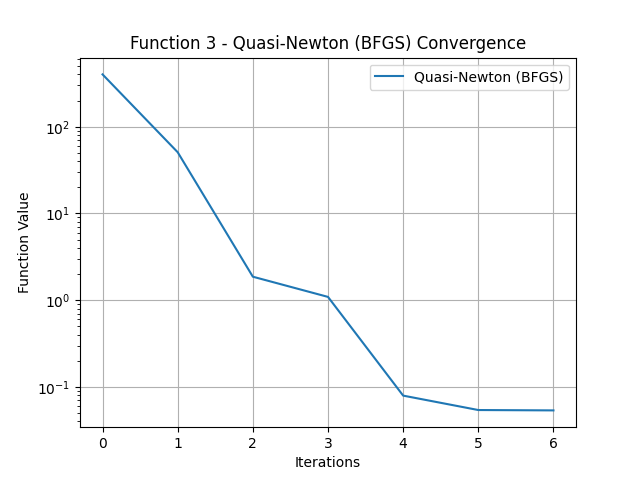
\includegraphics[width=0.18\textwidth]{/home/gobinda/My_Courses/QF/Optimization_Project2/artifacts/function_3_quasi-newton_(bfgs)_convergence.png}
   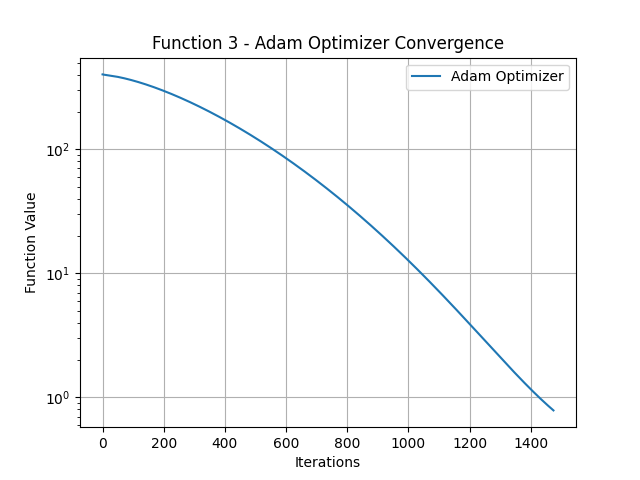
\includegraphics[width=0.18\textwidth]{/home/gobinda/My_Courses/QF/Optimization_Project2/artifacts/function_3_adam_optimizer_convergence.png}
   \caption{\small Convergence results for the Rosenbrock Function}
   \label{fig:rosenbrock_function_convergence}
\end{figure}

\begin{figure}[htbp]
   \centering
   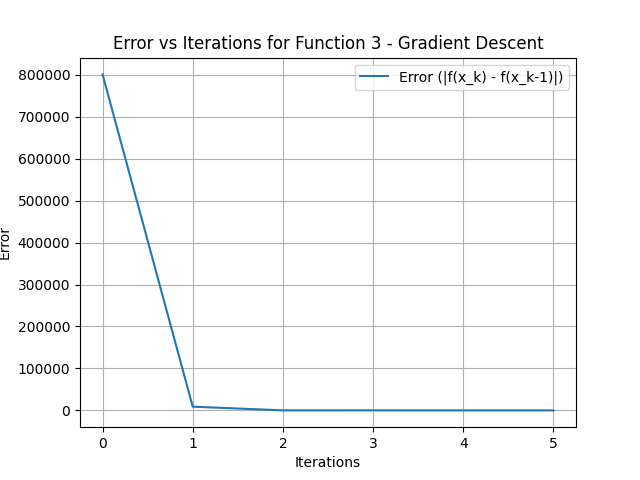
\includegraphics[width=0.18\textwidth]{/home/gobinda/My_Courses/QF/Optimization_Project2/artifacts/function_3_gradient_descent_errors.png}
   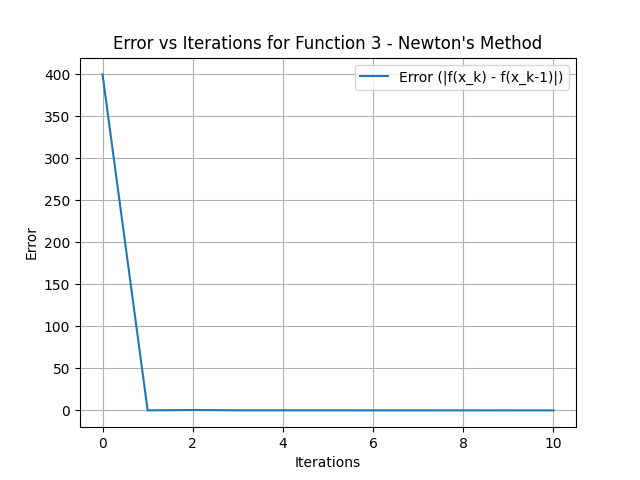
\includegraphics[width=0.18\textwidth]{/home/gobinda/My_Courses/QF/Optimization_Project2/artifacts/function_3_newton's_method_errors.png}
   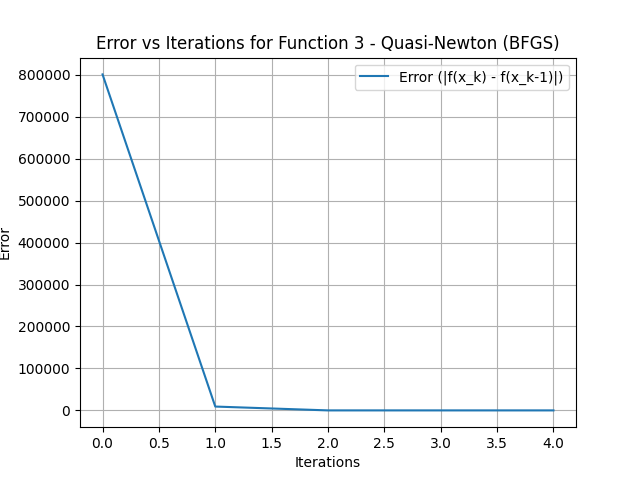
\includegraphics[width=0.18\textwidth]{/home/gobinda/My_Courses/QF/Optimization_Project2/artifacts/function_3_quasi-newton_(bfgs)_errors.png}
   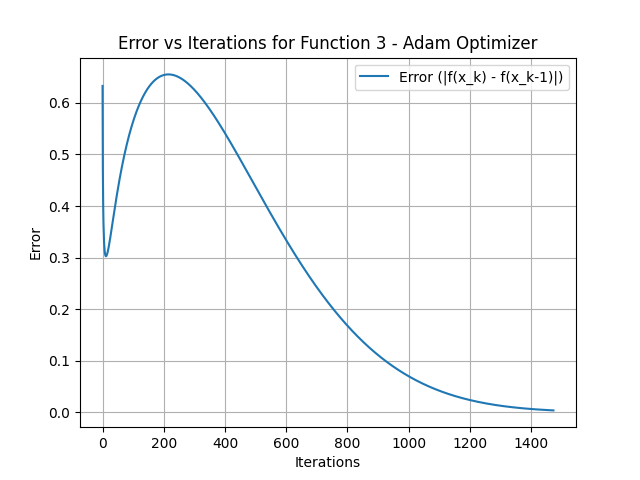
\includegraphics[width=0.18\textwidth]{/home/gobinda/My_Courses/QF/Optimization_Project2/artifacts/function_3_adam_optimizer_errors.png}
   \caption{\small Error results for the Rosenbrock Function}
   \label{fig:rosenbrock_function_errors}
\end{figure}

\FloatBarrier % Add this to ensure figures stay within the section

\subsubsection*{Explanation}
The Rosenbrock function is non-convex, posing a challenge for optimization methods. \textbf{Table \ref{tab:rosenbrock_function_results}} shows that Newton's Method achieved the lowest minimum in 10 steps, demonstrating robustness. Gradient Descent converged in 3 steps but to a higher minimum, indicating difficulty with the function's complexity. BFGS performed well, converging in 5 steps to a relatively low minimum. Adam required 1474 steps, showing it can handle non-convex functions but needs more iterations.
\textbf{Figure \ref{fig:rosenbrock_function_convergence}} illustrates convergence behavior. Newton's Method and BFGS show rapid convergence, while Gradient Descent and Adam exhibit gradual patterns.
\textbf{Figure \ref{fig:rosenbrock_function_errors}} shows error reduction over iterations. Newton's Method and BFGS exhibit rapid error reduction, whereas Gradient Descent and Adam need more iterations for similar accuracy.

\section{Conclusion} 
In conclusion, we tested four optimization methods: Gradient Descent, Newton’s Method, Quasi-Newton Method (BFGS), and the Adam Optimizer on three types of functions: Quadratic, Log Barrier, and Rosenbrock. We found that Newton’s Method and the Quasi-Newton Method (BFGS) generally performed better, especially for functions with clear shapes. In contrast, Gradient Descent and the Adam Optimizer needed more steps and careful adjustments to achieve good results. This highlights the importance of choosing the right optimization method based on the specific problem being solved.

\end{document}
